% ****** Start of file apssamp.tex ******
%
%   This file is part of the APS files in the REVTeX 4.1 distribution.
%   Version 4.1r of REVTeX, August 2010
%
%   Copyright (c) 2009, 2010 The American Physical Society.
%
%   See the REVTeX 4 README file for restrictions and more information.
%
% TeX'ing this file requires that you have AMS-LaTeX 2.0 installed
% as well as the rest of the prerequisites for REVTeX 4.1
%
% See the REVTeX 4 README file
% It also requires running BibTeX. The commands are as follows:
%
%  1)  latex apssamp.tex
%  2)  bibtex apssamp
%  3)  latex apssamp.tex
%  4)  latex apssamp.tex
%
\documentclass[%
 reprint,
%superscriptaddress,
%groupedaddress,
%unsortedaddress,
%runinaddress,
%frontmatterverbose, 
%preprint,
%showpacs,preprintnumbers,
%nofootinbib,
%nobibnotes,
%bibnotes,
 amsmath,amssymb,
 aps,
%pra,
%prb,
%rmp,
%prstab,
%prstper,
%floatfix,
]{revtex4-1}

\usepackage{graphicx}% Include figure files
\usepackage{dcolumn}% Align table columns on decimal point
\usepackage{bm}% bold math
\usepackage{multirow}
%\usepackage[showframe]{geometry}% http://ctan.org/pkg/geometry
\usepackage{lipsum}% http://ctan.org/pkg/lipsum
%\usepackage{hyperref}% add hypertext capabilities
%\usepackage[mathlines]{lineno}% Enable numbering of text and display math
%\linenumbers\relax % Commence numbering lines

%\usepackage[showframe,%Uncomment any one of the following lines to test 
%%scale=0.7, marginratio={1:1, 2:3}, ignoreall,% default settings
%%text={7in,10in},centering,
%%margin=1.5in,
%%total={6.5in,8.75in}, top=1.2in, left=0.9in, includefoot,
%%height=10in,a5paper,hmargin={3cm,0.8in},
%]{geometry}

\begin{document}

\preprint{APS/123-QED}

\title{NLU Project 2: Beyond seq2seq Dialogue Systems}% Force line breaks with \\
%\thanks{A footnote to the article title}%

\author{Florian Chlan}
 \email{fchlan@student.ethz.ch}
\author{Samuel Kessler}
 \email{sakessle@student.ethz.ch}
\author{Jovan Nikolic}
 \email{jovan.nikolic@gess.coss.ethz.ch}
 \author{Jovan Andonov}
 \email{andonovj@student.ethz.ch}
\affiliation{%
 ETH Zurich
}%
 %\altaffiliation[Also at ]{Physics Department, XYZ University.}%Lines break automatically or can be forced with \\

%\collaboration{MUSO Collaboration}%\noaffiliation

%\author{Charlie Author}
% \homepage{http://www.Second.institution.edu/~Charlie.Author}
%\affiliation{
% Second institution and/or address\\
% This line break forced% with \\
%}%
%\affiliation{
% Third institution, the second for Charlie Author
%}%
%\author{Delta Author}
%\affiliation{%
% Authors' institution and/or address\\
% This line break forced with \textbackslash\textbackslash
%}%

%\collaboration{CLEO Collaboration}%\noaffiliation

\date{\today}% It is always \today, today,
             %  but any date may be explicitly specified

\begin{abstract}
This article explores the implementation and performance of a vanilla seq2seq model for the purposes of language modeling and machine dialogue. Furthermore, extensions are made to improve on the performance of this baseline model. In particular: the dataset is extended to include the Cornell Movie-Dialog Corpus, words are embedded using word2vec, the seq2seq architecture is adapted to encapsulate global attention and additionally with an anti-language model to encourage diversity in the responses.


%\begin{description}
%\item[Usage]
%Secondary publications and information retrieval purposes.
%\item[PACS numbers]
%May be entered using the \verb+\pacs{#1}+ command.
%\item[Structure]
%You may use the \texttt{description} environment to structure your abstract;
%use the optional argument of the \verb+\item+ command to give the category of each item. 
%\end{description}
\end{abstract}

%\pacs{Valid PACS appear here}% PACS, the Physics and Astronomy
                             % Classification Scheme.
%\keywords{Suggested keywords}%Use showkeys class option if keyword
                              %display desired
\maketitle

%\tableofcontents

\section{\label{sec:level1}Introduction}
Deep learning has been very successful in tasks related to language modeling, machine translation, speech recognition and dialogue, with researchers edging closer to passing Turing's test. Today conversational agents mainly take the form of chat bots; used for a wide variety of tasks from ordering pizza to helping users cope with depression \cite{chatbothealth}.

The following report outlines several approaches to machine dialogue. The baseline seq2seq model (see \ref{seq2seq} for technical background) produced poor results; repeated generic answers for different input sentences such as \textit{"I don't know ."}, (see section \ref{results} for results). Subsequently, global attention (see \ref{globalattention} for technical background) was utilized to address the seq2seq model shortcomings. The global attention model was able to produce more sophisticated replies, however still suffered from generic replies, (see section \ref{results} for further details). To produce a more diverse set of responses an element of randomness was embedded into the dialogue machine (see \ref{antilmtb} for technical details and \ref{results} for results).

\section{\label{sec:level1}Technical Background}

\subsection{\label{sec:level2}Recurrent Neural Networks}

The recurrent neural network (RNN) is designed for learning sequences. In the dialogue context, an RNN recursively processes a sequence of embedded tokens (words or characters) $(w_1 \cdots w_T) \in V$, where $V$ is the vocabulary and $T$ is the input sequence length. At each time step the RNN updates its internal hidden state: $h_t = f(h_{t-1}, w_t) \in \mathbb{R}^{n}$, $n$ is chosen a priori. The function $f$ is usually a function of the form of an LSTM or GRU cell. The hidden state $h_t$ encapsulates all prior information regarding previous tokens. Hence, the hidden state can be projected via a softmax function onto the space of the vocabulary, of size $|V|$ for purposes of prediction. Crucially, the number of iterations where the network is unrolled needs to be known a priori: this presents a severe limitation for dialogue models.

\subsection{\label{sec:level2}Sequence to Sequence Models} \label{seq2seq}

Sequence to sequence (seq2seq) models learn how to map variable length sequences to sequences. Thus their ability to support conversational and translation models. The seq2seq model employs a first RNN network, the encoder, to map an input sequence to a fixed length vector $v \in \mathbb{R}^{n}$ and a second RNN network, the decoder, to map the vector to the target sequence. For additional details see \cite{seq2seq}.

\begin{figure}
  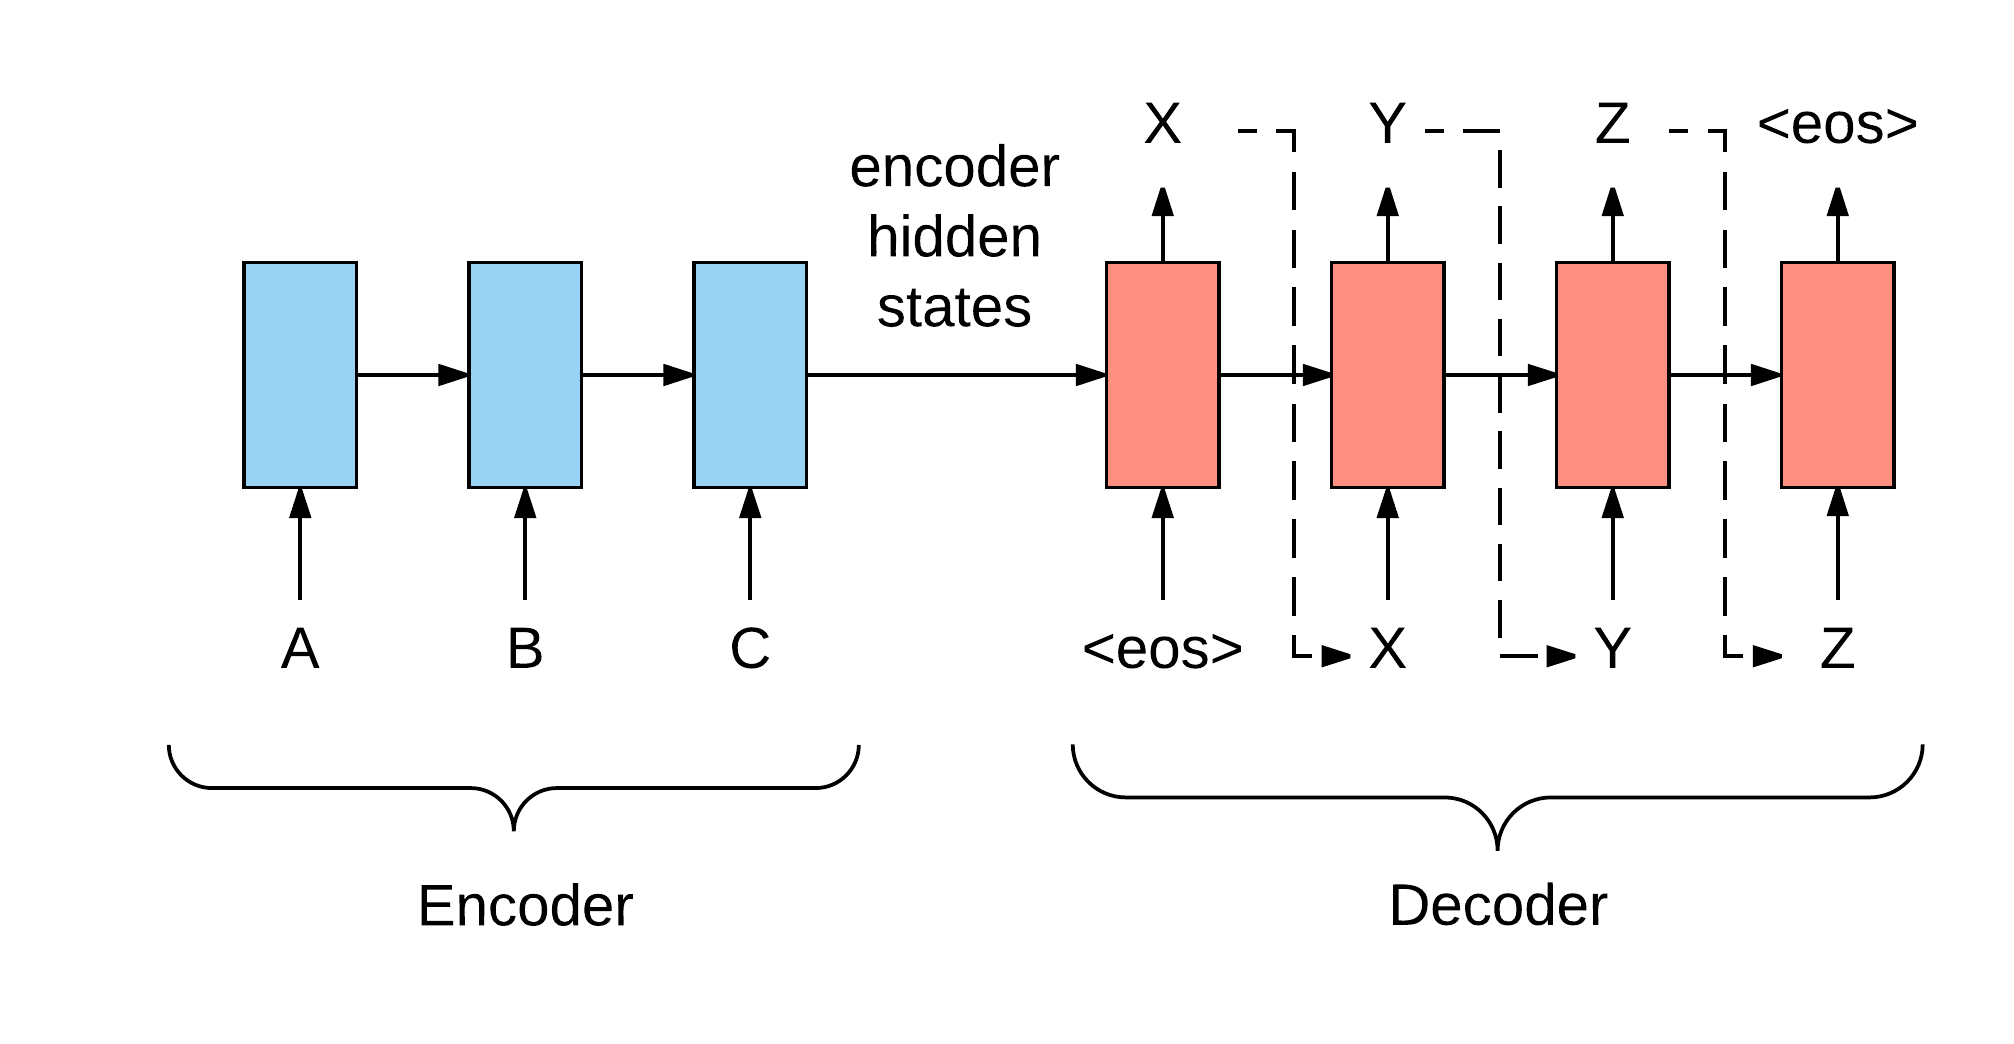
\includegraphics[width=9cm, height=5cm, keepaspectratio]{NLU_seq2seq.png}
  \caption{This is a sequence to sequence model for a conversational or translation model. $<$eos$>$ marks the end of a sentence.}
\end{figure}

%big!!!

%\begin{figure*}
%  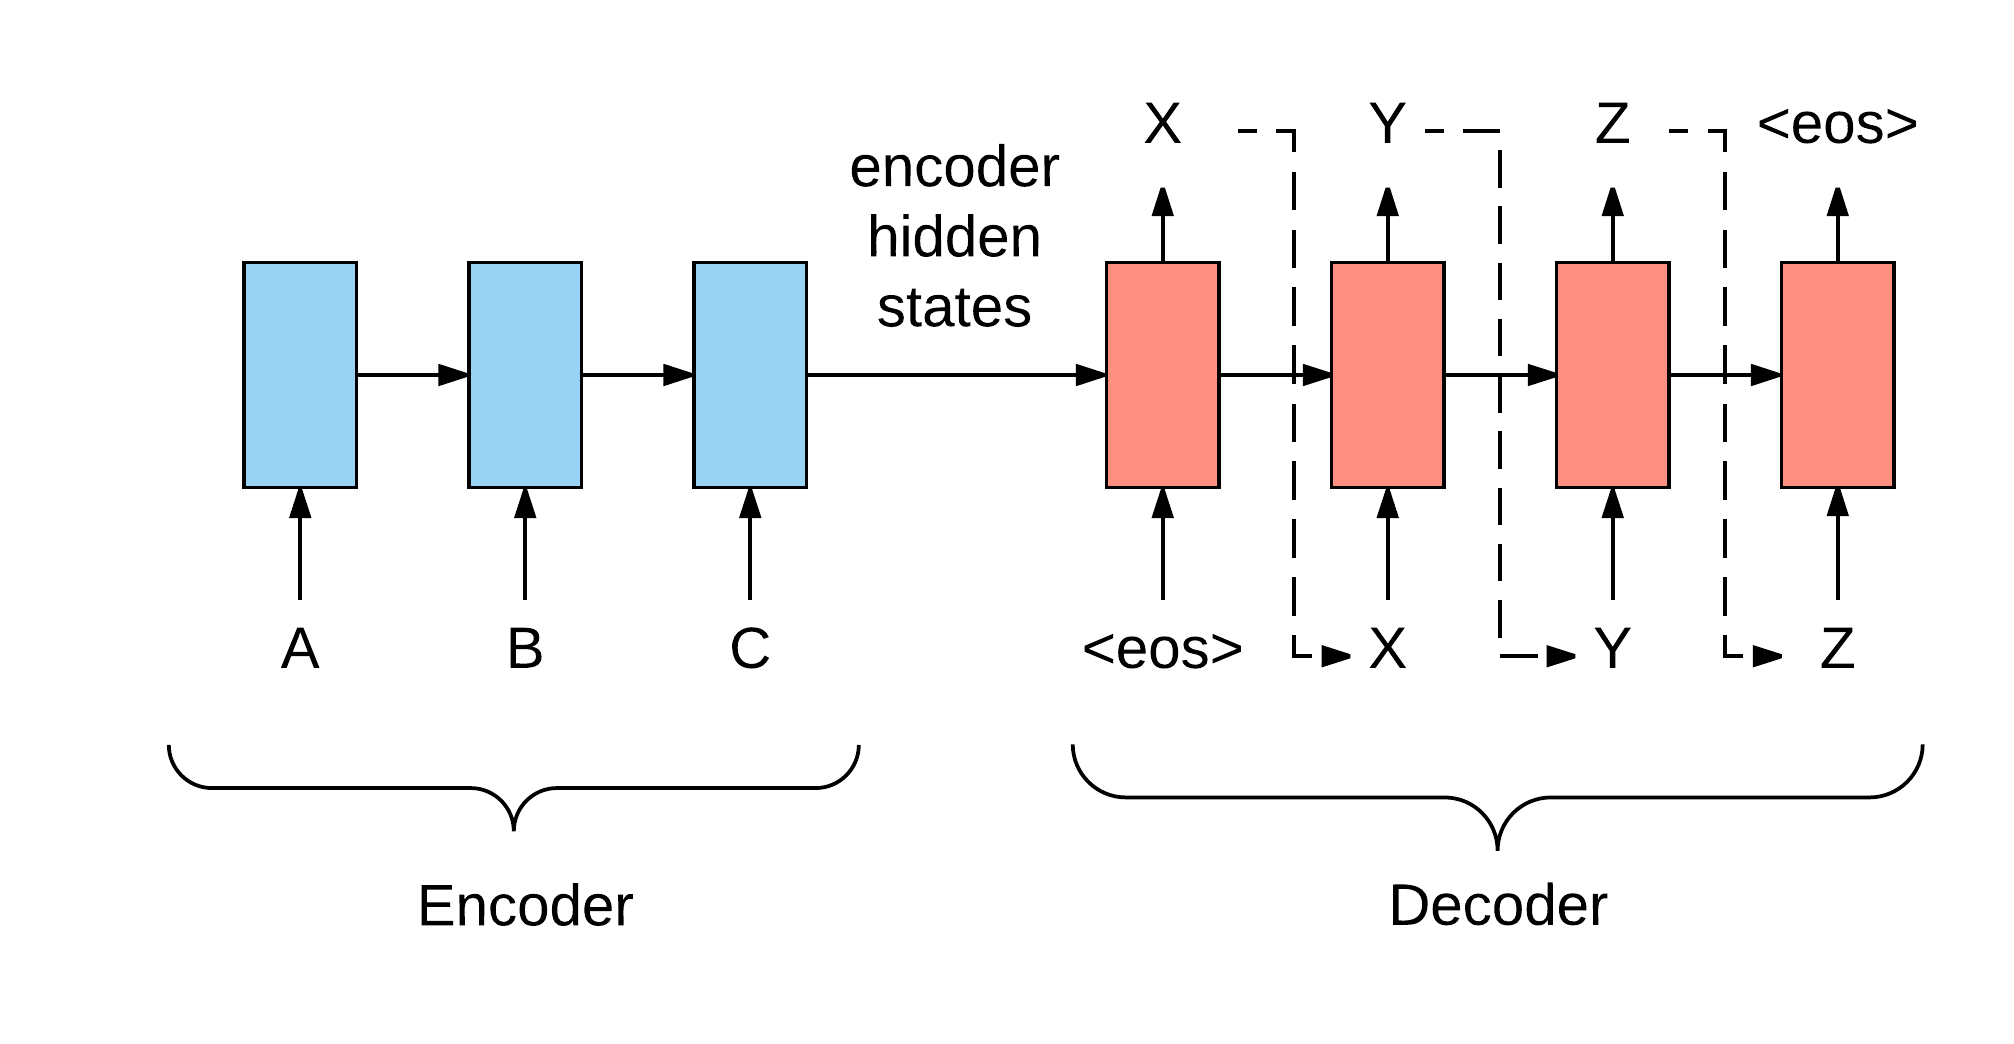
\includegraphics[width=\textwidth,height=\textheight, keepaspectratio]{NLU_seq2seq.png}
%  \caption{This is a tiger.}
%\end{figure*}


\subsection{\label{sec:level2}Global Attention} \label{globalattention}
For seq2seq models the encoder embeds the input sequence to a fixed length vector. This embedding presents a bottle neck. The performance of the decoder and the encoder degrades for longer sentence lengths.

Global attention aims to rectify this bottleneck by allowing the decoder to condition on all encoder hidden states. Intuitively, the decoder may choose certain parts of the encoded source sentence to focus on, when outputting a reply. 

The RNN graphical model defines a probability distribution $p(y)$ over the targets, which factorizes at every time step. Crucially, each conditional probability is conditioned on the context vector $c = f(\{h_1, \cdots h_{T}\}) \in \mathbb{R}^{n}$, where $f$ is a weighted sum.

\begin{equation}
p(y) = \prod_{t=1}^{T}p(y_t | \{y_1, \cdots y_{t-1} \}, c)
\end{equation}

For further details regarding global attention see \cite{globalattention}.

\begin{figure}
  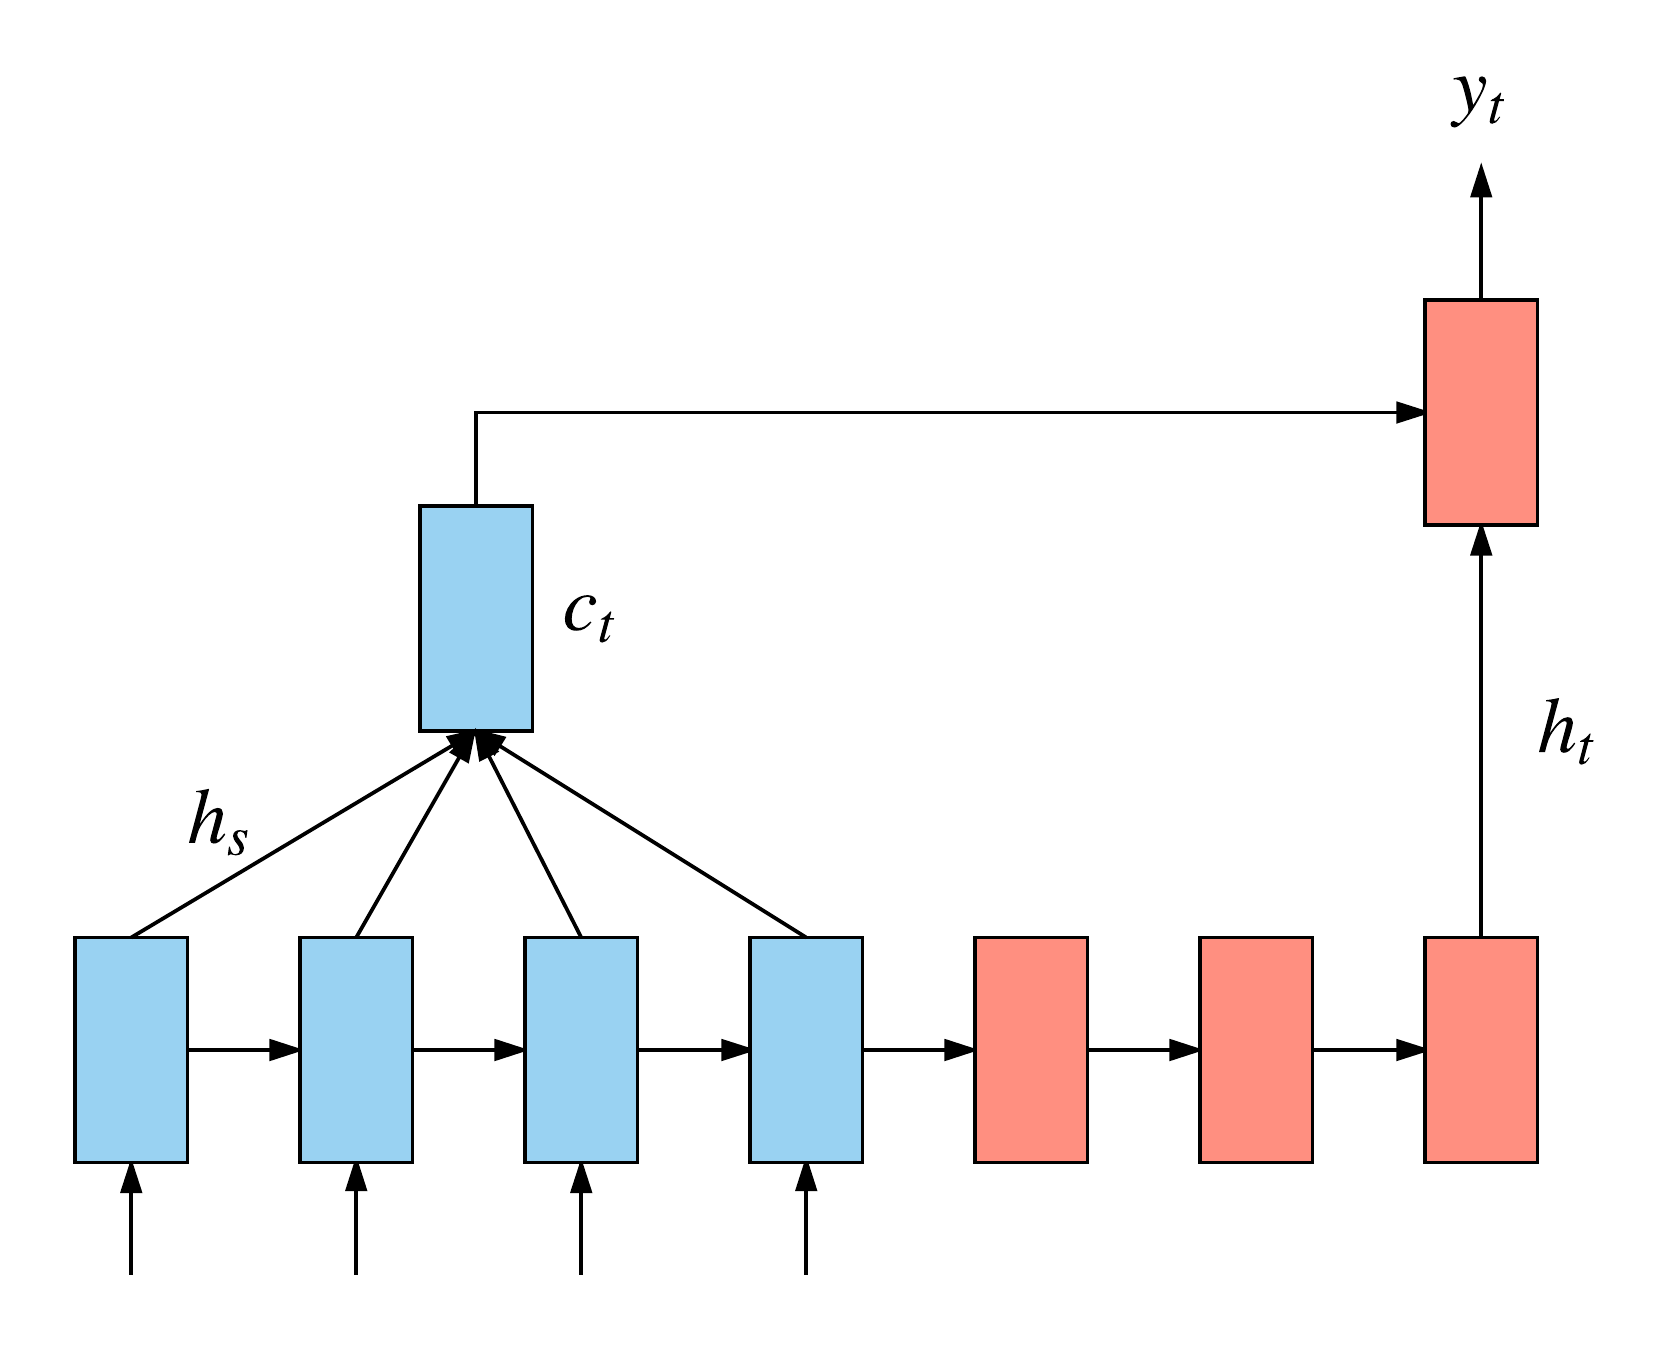
\includegraphics[width=8cm, height=5cm, keepaspectratio]{NLU_attention.png}
  \caption{Global attention model; a context vector, $c_t$, is calculated as a weighted average of source hidden states. The context vector is conditioned upon, on prediction of $y_t$ by the decoder. $h_s$ are the hidden states of the source sentences i.e. those of the encoder. $h_t$ are target hidden states i.e. those of the decoder.}
\end{figure}

\subsection{\label{sec:level2}Anti language model} \label{antilmtb}
To encourage more diverse responses for a dialogue machine a maximum mutual information is used as an objective function for the neural network, see \cite{antilm} for details. Targets are generated which maximize: 
\begin{equation} \label{antilmeqn}
P(T|S) - \lambda P(T)
\end{equation}

where $S$ is the source sentence, $T$ is the target sentence, $P(T|S)$ is the probability generated from the seq2seq decoder, $P(T)$ is the true distribution of targets, $\lambda$ is a penalization hyperparameter which only penalizes predictions up to $t=k$. 

\section{\label{sec:level1}Training Procedures}

The implementation was performed in TensorFlow. An existing TensorFlow implementation \cite{githubmatvey} formed the basis of the realization of the models introduced in this section. Cross entropy was used as the loss function. Adam optimization was employed in conjunction with the truncation of gradients larger than 10. Dropout with a probability of 0.5 was also introduced into the network to prevent overfitting.

\subsection{\label{sec:level2}Experiment Baseline}

\paragraph{Training data}
For all experiments a baseline training dataset from the Movie-DiC corpus was used. The corpus comprised over 392k conversation tuples. For sentences larger than 60 words long, the entire conversation tuple was removed from the training dataset. For each tuple, decoder targets were prepended with beginning-of-sentence tag, $<$bos$>$. Decoder targets were appended with the end-of-sentence tag, $<$eos$>$. Training was performed for 20 epochs.

\paragraph{Network variant experiments}
Experiments on the baseline were performed using a 1, 3 and 5 stacks of RNNs for the encoder and decoder which showed little improvement in the output. Additionally a bidirectional encoder was used, like in \cite{seq2seq}, with little improvement in the outputs. However, the paper was demonstrating a translation model and not a dialogue model, the author's discussion on the effectiveness of the bidirectional encoder is only relevant to a translation model. Network variant experiments were run for over 20 epochs with 20\% of the training data.

\paragraph{Implementation}
A vocabulary size of 10k was used out of over 67k unique words. Words were embedded into vectors in $\mathbb{R}^{200}$ using TensorFlow's "embedding\_matrix" via a simple partitioning of words into the embedding space. Single unidirectional RNNs were employed by the encoder and decoder. LSTM cells with a hidden state of size 512 were used as a basis of both encoder and decoder RNNs.

\subsection{\label{sec:level2}Global Attention}

\paragraph{Cornell Movie-Dialog Corpus}
The Cornell corpus was pre-processed to mimic the Movie-DiC dataset. The Cornell dataset comprised over 221k new sentences which could be added to the training dataset. Spaces between words and punctuation were added. All numbers were substituted with the $<$number$>$ tag. All names were replaced with a $<$person$>$ tag.

\paragraph{Word2vec}
The word2vec algorithm \cite{word2vec} was used for embedding words to vectors of size 200. word2vec was implemented with the Continuous Bag of Words (CBOW) algorithm, with a negative sampling of size 5. A vocabulary size of 10k was used. Words with a minimum frequency of 1 were embedded for 5 epochs. The embedding was trained on the Movie-DiC and Cornell corpses.

\paragraph{Implementation}
Global attention as described in \cite{globalattention} was implemented in TensorFlow version 1.0. Training was performed on 20 epochs.

\paragraph{Genres}
For each sentence in the Movie-DiC and Cornell data set, the genre of the original movie was prepended, as an additional feature for the network to learn from. Different genres will influence the dialogue of a movie.

\subsection{\label{sec:level2}Anti Language Model} \label{antilm}

\paragraph{Implementation} An existing implementation \cite{antilmgithub} inspired the anti language model. The Cornell data set, word2vec and global attention extensions were utilized. Inputs were fed into the encoder in reverse order, in line with \cite{antilmgithub}. A 3 layer encoder and decoder was used. The model was implemented in TensorFlow version 1.1.

\paragraph{Training} Scheduled sampling is used for training: with a probability of 0.75 the decoder feeds in the ground truth at time step $t$ and with a probability 0.25 it feeds in the softmax argmax from $t-1$ \cite{ss}. This is to improve the robustness of the predictions. Training was performed on 10 epochs.

\paragraph{Penalized Predictions}
For one particular conversation tuple, $P(T)$ in equation \ref{antilmeqn}, is estimated by passing as many $<$pad$>$ tokens into the encoder as there are input words \cite{antilmgithub}. Accordingly, $P(T)$ was estimated for each encoder input length. This probability can then be subtracted from the regular output probabilities over our vocabulary to penalize generic predictions and boost less generic predictions. The penalization is performed greedily at every time step. To add an extra degree of randomness the first token is sampled using a multinomial distribution, with the penalized logits as the underlying probability mass function. Doing this sampling for further than the first time step destroyed grammar in the predicted sentences. The hyperparameters $\lambda$ and $k$ were chosen manually, final values were 0.1 and k=4 i.e. the penalization was applied to the first 4 predicted tokens only. Higher values of $\lambda$ were also observed to destroy the grammar in the predicted sentences.

\section{\label{sec:level1}Results} \label{results}

\paragraph{Prediction}
For prediction in the network, the encoder is fed a source sentence which is subsequently encoded to a fixed length vector $\mathbb{R}^{200}$ and passed to the decoder in addition to a single $<$bos$>$ tag at $t=1$ to initiate the prediction process in the decoder RNN.

\paragraph{Model measurements}
The median perplexities have been calculated across the entire evaluation data sets for each model, table \ref{table:1}. The evaluation dataset is greater than 49k sentence pairs. Also, selected predictions have been chosen to demonstrate model performance, table \ref{table:2}.

The perplexity is calculated as follows:

\begin{equation}
Ppl = 2^{-\frac{1}{T} \sum^{T}_{t=1} log_{2}p(w_t | w_1 \cdots w_{t-1})}
\end{equation}

where $T$ is the length of the target sentence. The decoder is left to unroll until it reaches the $<$eos$>$ token, and $p(w_t | w_1 \cdots w_{t-1})$ is the probability of the ground truth token $w_t$ looked up from the softmax distribution output by the decoder at time $t$. Intuitively, the perplexity can be seen as a measure for how different a predicted sentence is to the evaluation set. The smaller the perplexity the greater the fidelity to the evaluation set.


\subsection{\label{sec:level2}Discussion}

Regarding perplexities, shown in table \ref{table:1}, the extensions made are seen to decrease the perplexities of our evaluation data set: the language model extensions are seen to improve learning. Significant improvements were observed for the anti language model predictions. However the reported perplexities are an order of magnitude greater than perplexities presented in recent conference papers \cite{antilm} \cite{persona}. 

The observed predictions in table \ref{table:2} are more sobering; a significant proportion of the baseline predictions are very generic e.g. $<$person$>$ . $<$eos$>$. The attention model extensions provide slightly more variety in the replies, nonetheless far from the mark, in comparison to the ground truth. Amusingly, the anti language model provides more diversity in the vocabulary of the reply, at the cost of a meaningful and grammatically correct replies.

\begin{table}[h!]
\centering
\begin{tabular}{| m{20em} | m{1cm}| } 
 \hline
 Model & Ppl \\ [0.5ex] 
 \hline
 Baseline & 373  \\ 
 \hline
 Baseline + Cornell + word2vec + global attention & 327  \\ 
 \hline
 Baseline + Cornell + word2vec + global attention + genres & 337 \\ [1ex] 
 \hline
 Baseline + Cornell + word2vec + global attention + anti language model & 271 \\ 
 \hline
\end{tabular}
\caption{Results: median perplexities across the validation data set for stated models.}
\label{table:1}
\end{table}


\begin{table*}[t]
\centering
\begin{tabular}{| m{8cm} | m{8cm}| } 
 \hline
 Context & Response \\
 \hline
 \multirow{5}{8cm}{goodbye , young fellow . we ' ll see what we can do .
} & GT: i ' m not worried . everything will be fine . the old team together . nothing can stop us . she turns and walks out of the shot . <person> stands for a second watching her , then turns to his assistant . \\ 
 & B: $<$person$>$ . $<$eos$>$ \\
 & BA: bathroom . $<$eos$>$ \\
 & BAG: i ' m not going to see you again . $<$eos$>$ \\
 & BA+antilm: going earth ve sing ? $<$eos$>$\\
 \hline
  \multirow{5}{8cm}{me either . i wish i could . . but . want me to shut these , sun comes in pretty strong in the morning .} & GT: sure . . . thanks . . . \\ 
 & B: $<$person$>$ . $<$eos$>$ \\
 & BA: $<$person$>$ . $<$eos$>$ \\
 & BAG: you ' re right . $<$eos$>$ \\
 & BA+antilm: yourselves best , saturday , i ' retreat a $<$unk$>$ . $<$eos$>$\\
 \hline
\multirow{5}{8cm}{well , i don ' t know anyone named obi- wan , but old ben lives out beyond the dune sea . he ' s kind of a strange old hermit . $<$continued\_utterance$>$ i wonder who she is . it sounds like she ' s in trouble . i ' d better play back the whole thing .} & GT: he says the restraining bolt has short circuited his recording system . he suggests that if you remove the bolt , he might be able to play back the entire recording . \\ 
 & B: $<$person> . $<$eos$>$  \\
 & BA: $<$person$>$ . $<$eos$>$ \\
 & BAG: you ' re a very attractive woman . $<$eos$>$ \\
 & BA+antilm: fame $<$person$>$ , $<$person$>$ . $<$eos$>$ \\
 \hline
 \multirow{5}{8cm}{what ' ve you done ?} & GT: nothing . \\ 
 & B: i ' m going to get a job . $<$eos$>$ \\
 & BA: i ' m not sure . $<$eos$>$ \\
 & BAG: i ' m not sure . $<$eos$>$ \\
 & BA+antilm: away and notice about the $<$unk$>$ . $<$eos$>$\\
 \hline
 \multirow{5}{8cm}{nobody . it used to be that sex was the only free thing in the world . no longer . <person> , alimony . all financial . <person> ' s an illusion .} & GT: it ' s the only illusion that counts .\\ 
 & B: $<$person$>$ . $<$eos$>$\\
 & BA: $<$person$>$ . $<$eos$>$\\
 & BAG: you ' re a monster . $<$eos$>$\\
 & BA+antilm: dude more problems there . $<$eos$>$\\
 \hline
 \multirow{5}{8cm}{sometimes i get boners so big i can ' t hide them . and then i get nervous and my heart starts pounding , and it all just , like , feeds my boner . it just becomes this . thing . that ' s attached to me . and it won ' t go away .} & GT: just imagine if girls weren ' t $<$unk$>$ out by our $<$unk$>$ and they actually wanted to see `em , like this shit .\\ 
 & B: $<$person$>$ , i ' m sorry . $<$eos$>$ \\
 & BA: i ' ll kill you . $<$eos$>$ \\
 & BAG: you ' re not going to kill me . $<$eos$>$\\
 & BA+antilm: not interested sing throws . $<$eos$>$ \\
 \hline
\end{tabular}
\caption{Dialogues. GT is the ground truth, B is the baseline, BA is the baseline model + word2vec + Cornell + global attention. BAG is BA + genres. BA+antilm: BA + anti language model.}
\label{table:2}
\end{table*}


In general, the results are poor for the sophistication of the system. The perplexity values are high and a significant proportion of the predicted sentences from the decoder are very generic. Despite reusing working code from \cite{githubmatvey} and \cite{antilmgithub} it is accepted that there might be a bug tarnishing the experiments described above.

\subsection{\label{sec:level2}Improvements}

A larger corpus and longer training times would improve results, state of the art models are based on the order of $10^6-10^7$ sentence pairs \cite{localattention} \cite{antilm}. The potential bug needs to be addressed. Additionally incorporating reinforcement learning \cite{rf} and in particular, beam-search would lead to improved results \cite{beamsearch}.


\begin{thebibliography}{9}

\bibitem{chatbothealth} 
Stanford’s Woebot is a therapy chatbot for depression and anxiety - Business Insider. (n.d.). Retrieved June 9, 2017, from http://uk.businessinsider.com/stanford-therapy-chatbot-depression-anxiety-woebot-2017-6?r=US\%5C\&IR=T
 
\bibitem{seq2seq} 
Sutskever, I., Vinyals, O., \& Le, Q. V. (2014). Sequence to Sequence Learning with Neural Networks. Retrieved from http://arxiv.org/abs/1409.3215.

\bibitem{globalattention} 
Bahdanau, D., Cho, K., \& Bengio, Y. (n.d.). NEURAL MACHINE TRANSLATION BY JOINTLY LEARNING TO ALIGN AND TRANSLATE. Retrieved from https://arxiv.org/pdf/1409.0473.pdf

\bibitem{githubmatvey} 
Matvey Ezhov
https://github.com/ematvey/tensorflow-seq2seq-tutorials

\bibitem{cornell} 
Cornell Movie - Dialog Corpus
https://www.cs.cornell.edu/\~{}cristian/Cornell\_Movie-Dialogs\_Corpus.html

\bibitem{word2vec} 
Mikolov, T., Sutskever, I., Chen, K., Corrado, G., \& Dean, J. (n.d.). Distributed Representations of Words and Phrases and their Compositionality. Retrieved from http://web2.cs.columbia.edu/\~{}blei/seminar/2016\_discrete\_data/ \\
readings/MikolovSutskeverChenCorradoDean2013.pdf

\bibitem{ss}
Bengio, S., Vinyals, O., Jaitly, N., \& Shazeer, N. (n.d.). Scheduled Sampling for Sequence Prediction with Recurrent Neural Networks. Retrieved from https://papers.nips.cc/paper/5956-scheduled-sampling-for-sequence-prediction-with-recurrent-neural-networks.pdf

\bibitem{antilmgithub}
Marsan-ma
https://github.com/Marsan-Ma/tf\_chatbot\_seq2seq\_antilm

\bibitem{antilm}
Li, J., Galley, M., Brockett, C., Gao, J., \& Dolan, B. (2016). A Diversity-Promoting Objective Function for Neural Conversation Models. Retrieved from https://arxiv.org/pdf/1510.03055.pdf

\bibitem{localattention}
Luong, M.-T., Pham, H., \& Manning, C. D. (2015). Effective Approaches to Attention-based Neural Machine Translation. Retrieved from https://arxiv.org/pdf/1508.04025.pdf

\bibitem{persona}
Li, J., Galley, M., Brockett, C., Spithourakis, G. P., Gao, J., \& Dolan, B. (n.d.). A Persona-Based Neural Conversation Model. Retrieved from https://arxiv.org/pdf/1603.06155.pdf

\bibitem{rf}
Li, J., Monroe, W., Ritter, A., Galley, M., Gao, J., \& Jurafsky, D. (n.d.). Deep Reinforcement Learning for Dialogue Generation. Retrieved from https://arxiv.org/pdf/1606.01541.pdf

\bibitem{beamsearch}
Wiseman, S., \& Rush, A. M. (n.d.). Sequence-to-Sequence Learning as Beam-Search Optimization. Retrieved from https://arxiv.org/pdf/1606.02960.pdf

\end{thebibliography}

\end{document}
%
% ****** End of file apssamp.tex ******